\documentclass{article}
\usepackage[utf8]{inputenc}
\usepackage{geometry}
\usepackage{pdfpages}
\usepackage{graphicx}
\usepackage{filecontents}

\graphicspath{{images/}}
\geometry{
	a4paper,
	total={170mm,257mm},
	left=20mm,
	top=20mm,
}
\usepackage{graphicx}
\usepackage{titling}
\usepackage[american,RPvoltages]{circuiTikz}
\usepackage{tikz, tikz-cd}
\usepackage{pgfplots}
\usepackage{siunitx}
\usepackage{float}
\usepackage{enumitem}
\usepackage{amsmath,amsfonts,stmaryrd,amssymb} % Math packages
\usepackage{schemabloc}
\usetikzlibrary{circuits}
\usetikzlibrary{positioning}
\title{Generador de Onda Cuadrada}
\author{Rodrigo}
\date{Agosto 2024}

\usepackage{fancyhdr}
\fancypagestyle{plain}{%  the preset of fancyhdr 
	\fancyhf{} % clear all header and footer fields
	\fancyfoot[L]{\thedate}
	\fancyhead[L]{Osciladores}
	\fancyhead[R]{\theauthor}
}
\makeatletter
\def\@maketitle{%
	\newpage
	\null
	\vskip 1em%
	\begin{center}%
		\let \footnote \thanks
		{\LARGE \@title \par}%
		\vskip 1em%
		%{\large \@date}%
	\end{center}%
	\par
	\vskip 1em}
\makeatother

\usepackage{lipsum}  
\usepackage{cmbright}

\begin{document}
	
	\maketitle
	
	\noindent\begin{tabular}{@{}ll}
		Author & \theauthor\\
	\end{tabular}
	
	\section*{Resumen}
Un generador de onda cuadrada puede ser generado si un amplificador operacional es forzado a oscilar repetidamente entre la saturación positiva $+V_{sat}$ y la saturación negativa $-V_{sat}$. Esto se puede lograr conectando un multivibrador biestable (o Schmitt Trigger) con un circuito RC en el lazo de realimentación. La implementación del circuito se muestra en la figura 1(a).

\begin{figure}[H]
	\centering	
	\begin{tikzpicture}[scale=0.8]
		\ctikzset{bipoles/thickness=3}
		\ctikzset{monopoles/vcc/arrow={Stealth[width=6pt,length=9pt]}}
		\ctikzset{monopoles/vee/arrow={Stealth[width=6pt,length=9pt]}}
		\draw (0,0) to[C, -*, l=$C$] ++(3,0) node[above]{$v_c$} coordinate (c1)
		      to[short] ++(0,-3) node[above right]{$v_{-}$}
		      to[short] ++(1.5,0) coordinate (p1);
		\draw (p1) node[op amp, anchor=-](OA){};
		\draw (c1) to[R, l=$R$] (c1 -| OA.out) -- (OA.out);
		\draw (OA.+) to[short] ++(-1.5,0) node[below right]{$v_{+}$} coordinate (p3)
		to[short] ++(0,-3) coordinate(p2);
		\draw (p2) to[R, l_=$R_2$] (p2 -| OA.out) -- (OA.out);
		\draw (OA.out) to[short, *-o] ++(1,0) node[right]{$v_{o}$};
		\draw (p3) to[R, *-*, l=$R_1$] ++(-3,0);
		\draw(0,0) to [short] ++(0,-6) node[ground]{};
		\draw(OA.up) to[short] ++(0,0.4) node[vcc](VCC){$+V_{CC}$};
		\draw(OA.down) to[short] ++(0,-0.4) node[vee](VEE){$-V_{EE}$};
		\node[anchor=west] at (2.5,-9){$(a) \, circuito$};
		\node[anchor=west] at (12,-9){$(b) \, Formas \, de \, onda$};
		\node[anchor=west] at (7,-15){$(c) \, Circuito \, equivalente$};
		\draw (OA.+) to[open, v=$v_d$] (OA.-);
		
		\draw (7,-10) coordinate (t1) to[C, v>=$v_{th}$, l=$C$] ++(0,-3) node[ground]{};
		\draw (t1) to[R, -o, i^<=$i_C$, l=$R$] ++(5,0) coordinate(t2);
		\draw (t2) to[open, v=$V_{sat}$] ++(0,-4);      
		\draw (8.5,-10) to[open, v = $v_C$] ++(0,-4);
	    \pgfplotsset{width=9cm,compat=1.18}
		\begin{axis}[xshift=11cm,
			yshift=-7cm,
			clip=false,
			axis y line=left,
			axis x line=middle, 
			xmin=0,xmax=3.5,
			ymin=-1.5,ymax=1.5,
			xlabel=$t$,
			ylabel=$v$,
			axis y line= center,
			xtick={3.14,6.28},
			xticklabels={$\pi\,$, $\,\,\,2\pi$},
			ytick={-1, -0.4187, 0, 0.418, 1},
			yticklabels={$V_{sat} = V_{EE}$,$-V_{th}$,$0$,$+V_{th}$,$V_{sat} = V_{CC}$},
			]
			\addplot+[thick,mark=none,const plot]
			coordinates {(0,0) (0,1) (1,-1) (2,-1) (2,1) (3,1) (3,-1) (3.4,-1)};
			\addplot[smooth, magenta, mark=none, domain=0:1, samples=200] {-(exp(-x/0.4) - 0.5)};
			\addplot[smooth, magenta, mark=none, domain=0.992:2, samples=200] {(exp(-(x-1)/0.4) - 0.6)};
			\addplot[smooth, magenta, mark=none, domain=1.993:3, samples=200]{-(exp(-(x-2)/0.4) - 0.5)};
		    \addplot[color = black, dashed, thick] coordinates {(0,0.418) (3, 0.418)};
		    \addplot[color = black, dashed, thick] coordinates {(0,-0.5) (3, -0.55)};
			\draw[<-](0.5, 1.05)--(0.7, 1.2); %vo
			\draw[<-](1.2, 0.1)--(1.4, 0.3); %vc
			\node[anchor=west] at (axis cs:0.6,1.3){$v_O$};
			\node[anchor=west] at (axis cs:1.35,0.3){$v_c$};
			\draw[->] (1.6,-0.8) node[left=-0.5mm]{$t_2$}-- (2,-0.8);
			\draw[<-] (1,-0.8) -- (1.4,-0.8);
			\draw[->] (0.6,-0.8) node[left=-0.6mm]{$t_1$}-- (1,-0.8);
			\draw[<-] (0,-0.8) -- (0.4,-0.8);
			\draw[->|] (1.2,-1.2) node[left=1mm]{$T$}-- (2,-1.2);
			\draw[<-] (0,-1.2) -- (0.8,-1.2);
			
			
		\end{axis}
	;\end{tikzpicture}
	\caption{}	
	\label{fig:figura2}
\end{figure}

\noindent Este tipo de generador de onda cuadrada es conocido como \textbf{multivibrador astable} o de \textit{marcha libre} porque la salida no tiene un estado estable. La salida del amplificador operacional estará en la saturación positiva o negativa, dependiendo de si $v_d$ es positivo o negativo. \\

\noindent Asumimos que el voltaje en el capacitor es cero, el voltaje en la terminal inversora será de cero inicialmente, esto es, $v_{-} = 0$ en el instante en que la fuente de alimentación se conecte. Sin embargo, en ese mismo instante, el voltaje $v_{+}$ en la terminal no inversora tendrá un pequeño valor que dependerá del voltaje de offset $V_{OS}$, esto es:

\begin{align}
	v_d = v_{+} - v_{-} = V_{OS}
\end{align}

El cuál tendrá un valor positivo. Sin embargo, $v_d$ será amplificado como resultado de la muy alta ganancia del amplificador operacional (típicamente de $2 \cdot 10^5$) y llevará la salida del amplificador operacional a saturación positiva ($+V_{sat}$), como resultado, el capacitor $C$ se estará cargando a través de la resistencia $R$. No obstante, tan pronto como el voltaje en $C$, el cual es igual a $v_{-}$ sea ligeramente mayor a $v_{+}$, entonces $v_d = v_{+} - v_{-}$ se volverá negativo y la salida del amplificador conmutará a saturación negativa.
La operación del circuito puede dividirse en dos modos: el modo 1 para $v_d > 0$ y el modo 2 para $v_d < 0$ \\

\noindent Durante el modo 1, $v_d > 0$ por lo que el voltaje de salida del amplificador operacional se encontrará en saturación positiva $+V_{sat}$. El voltaje en $v_+$ es:

\begin{align}
	v_{+} = \frac{R_1}{R_1 + R_2}(+V_{sat})
\end{align}

El capacitor $C$ comenzará a cargarse hacia $+V_{sat}$ a través de $R$. Tan pronto como el voltaje a través de $C$ sea ligeramente mayor que $v_{+}$, entonces $v_d = v_{+} - v_{-}$ se volverá negativo y la salida del amplificador se verá forzada a conmutar a saturación negativa.

Durante el modo 2, $v_d < 0$ y la salida del amplificador se encontrará en saturación negativa $-V_{sat}$. El voltaje $v_{+}$ sigue la regla del divisor de voltaje, por lo tanto:

\begin{align}
	v_{+} = \frac{R_1}{R_1 + R_2}(-V_{sat})
\end{align}

El voltaje $v_{+}$ actúa como un voltaje de referencia. El voltaje del capacitor $v_{-}$ intenta seguir a $v_{+}$. Sin embargo, tan pronto como la magnitud de $v_{-}$ se vuelve mayor que la de $v_{+}$, $v_{+}$ cambiará su polaridad. Como resultado, la salida oscilará desde un valor positivo a un valor negativo y viceversa. La forma de onda del voltaje de salida se muestra en la figura 1(b). \\

\noindent El circuito equivalente durante el periodo de carga asumiendo que $+V_{sat}$ es el voltaje de salida  y el capacitor tiene un voltaje incial de $-v_{th}$ durante el modo 1, se muestra en la figura 1(c).

\noindent El voltaje en el capacitor está dado por:

\begin{align}
	v_c(t) = v(\infty) + [v(0) - v(\infty)]e^{-\frac{t}{\tau}}
\end{align}

\noindent Donde $v(\infty) = +V_{sat}$ y $v(0) = -V_{th}$, por lo tanto

\begin{align}
	v_c(t) = V_{sat} - [V_{th} + V_{sat}]e^{-\frac{t}{RC}}
\end{align}

\noindent En $t = t_1$ el capacitor se carga hasta $v_{th}$, por tanto, obtenemos

\begin{align}
	V_{th} - V_{sat} &= - [V_{th} + V_{sat}]e^{-\frac{t}{RC}} \nonumber \\
	V_{sat} - V_{th} &= [V_{th} + V_{sat}]e^{-\frac{t}{RC}} \nonumber \\
	e^{-\frac{t}{RC}} &= \frac{V_{sat} - V_{th}}{V_{th} + V_{sat}} \nonumber \\
	-\frac{t}{RC} &= \ln{\frac{V_{sat} - V_{th}}{V_{th} + V_{sat}}} \nonumber \\
	t_1 &= -RC\ln{\frac{V_{sat} - V_{th}}{V_{th} + V_{sat}}} \nonumber \\
	t1 &= -RC\ln{\frac{V_{sat} - \frac{R_1}{R_1 + R_2}V_{sat}}{V_{sat} +\frac{R_1}{R_1 + R_2}V_{sat}}  } \nonumber \\
	t_1 &= -RC \ln {\frac{1 - \frac{R_1}{R_1 + R_2}}{1 + \frac{R_1}{R_1 + R_2}}} \nonumber \\
	t_1 &= -RC \ln{\frac{ \frac{R_2}{R_1 + R_2} }{ \frac{2R_1 + R_2}{R_1 + R_2} }} = -RC \ln{\frac{R_2}{2R_1 + R_2}} \nonumber \\
	t_1 &= -RC \left[ \ln {R_2} - \ln {(2R_1 + R_2)} \right] = RC \left[ \ln {(R_2 + 2R_1)} - \ln{R_2} \right] \nonumber
\end{align}

\begin{align}
	t_1 = RC \ln \left( \frac{R_2 + 2R_1}{R_2} \right)
\end{align}
 
 \noindent El periodo $T$ del voltaje de salida está dado por:
 
 \begin{align}
 	T = t_1 + t_2 = 2t_1 = 2RC \ln \left( \frac{R_2 + 2R_1}{R_2} \right)
 \end{align}
 
\noindent Así, la frecuencia de oscilación $f_0$ del voltaje de salida es:

\begin{align}
	f_0 = \frac{1}{T} = \frac{1}{ 2RC \ln \left( \frac{R_2 + 2R_1}{R_2} \right) }
\end{align}

\noindent Si queremos aproximar la frecuencia de salida a $f_0 = \frac{1}{2RC}$ debemos hacer que el término $\ln[(R_2 + 2R_1)/R_2]$ sea igual a $1$, por lo tanto:

\begin{align}
	\ln \left( \frac{R_2 + 2R_1}{R_2} \right) = 1 \nonumber \\
	\frac{R_2 + 2R_1}{R_2} = e = 2.7183 \nonumber \\
	R_2 + 2R_1 = 2.7183R_2 \nonumber \\
	1.7183R_2 = 2R_1 \nonumber
\end{align}

Es decir:

\begin{align}
	R_2 = 1.164R_1
\end{align}

Cumpliendo con estas condiciones la frecuencia de oscilación es:

\begin{align}
	f_0 = \frac{1}{2RC}
\end{align}

\newpage

\section*{Ejemplo de diseño}
Diseñe un generador de onda cuadrada o multivibrador astable usando el amplificador operacional LT1220 de Analog Devices para obtener una señal cuadrada a una frecuencia de $\qty{1}{\kilo\hertz}$. Use la condición $R_2 = 1.164R_1$, sea $C = 0.01uF$

\begin{figure}[H]
	\centering
	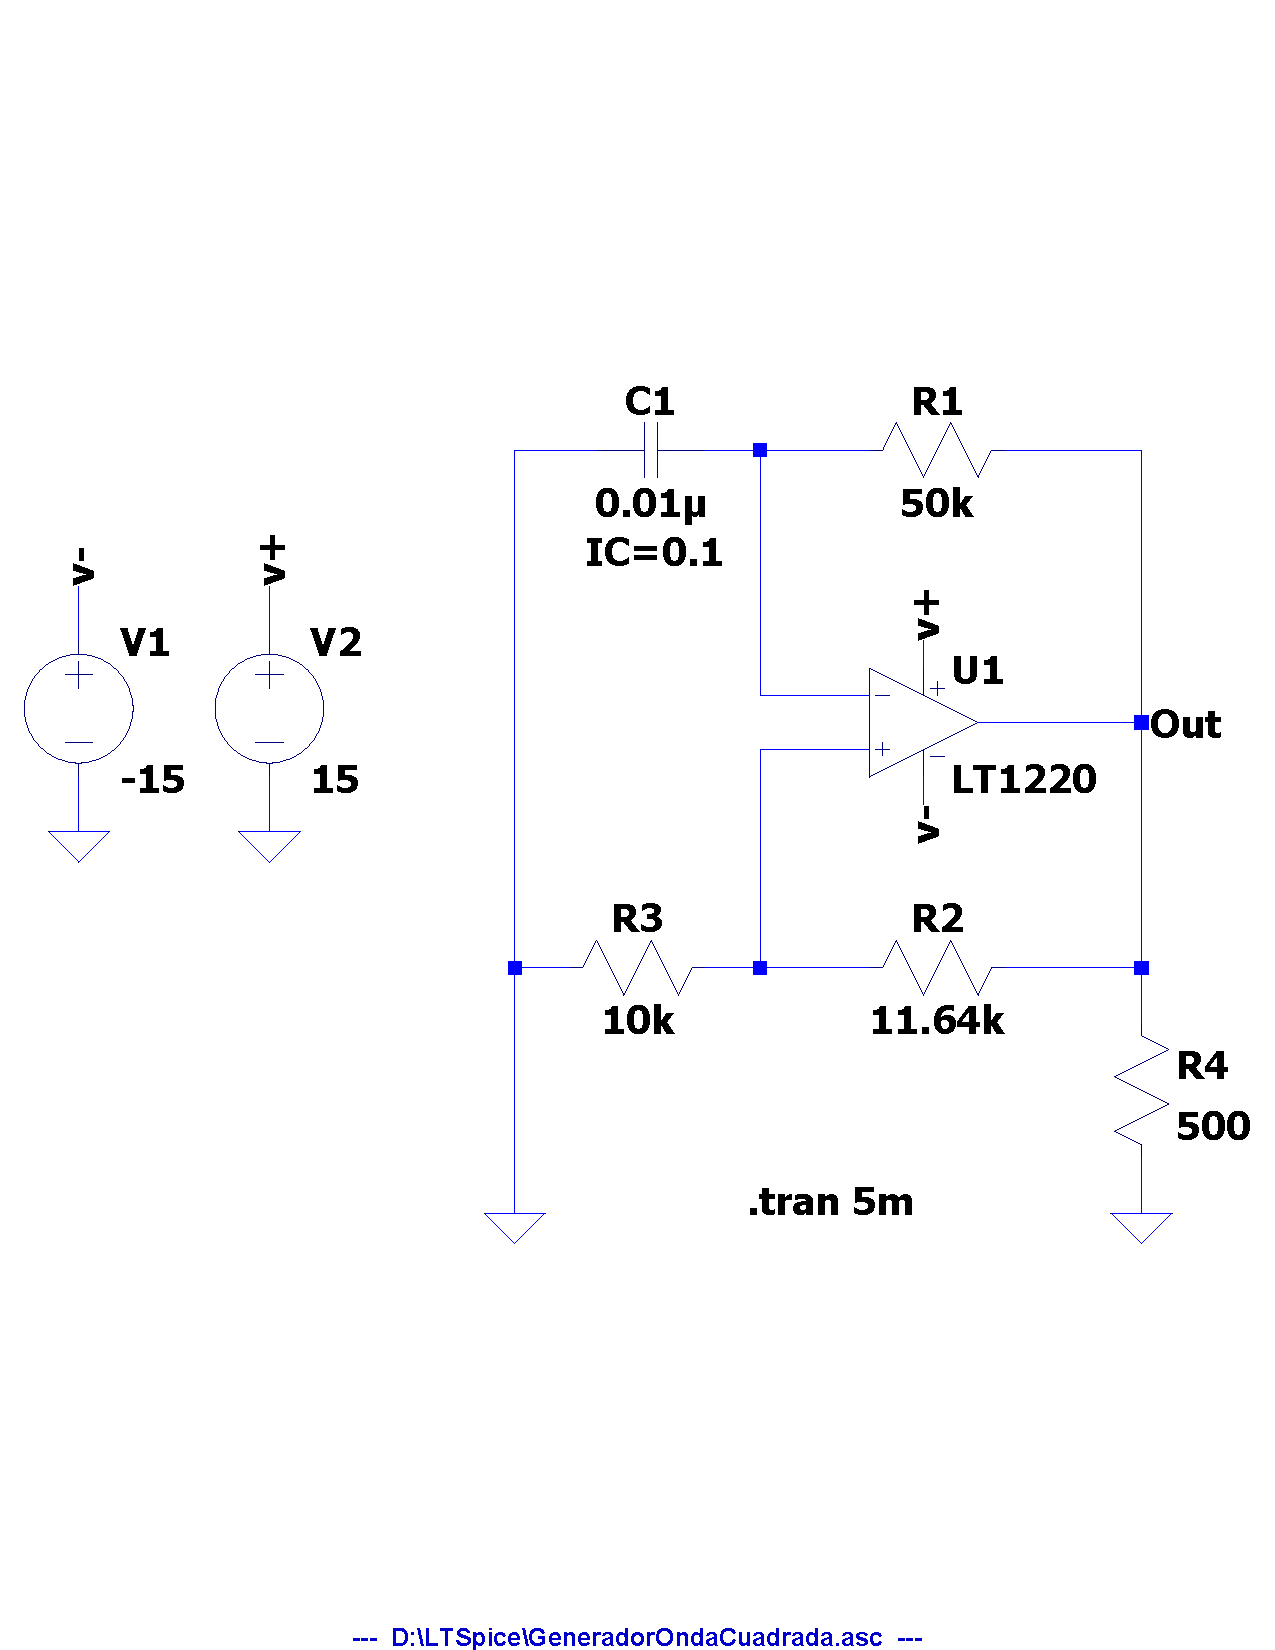
\includegraphics[clip, trim=0cm 6.5cm 0cm 6cm, scale=0.55]{picture}
	\caption{}	
	\label{fig:figura5}
\end{figure}

Despejamos $R$ de la ecuación (10) para obtener

\begin{align}
	R = \frac{1}{2f_0 C}
\end{align}

Reemplezando el valor de $C$ y la frecuencia en (10) obtenemos

\begin{align}
	R = \frac{1}{2(\qty{1}{\kilo\hertz})(\qty{0.01}{\micro\farad})} = \qty{50}{\kilo\ohm} \nonumber
\end{align}


\noindent Elegimos un valor arbitrario para $R_1$ , por ejemplo, sea $R_1 = \qty{10}{\kilo\ohm}$, por lo tanto
\begin{align}
	R_2 = 1.164R_1 = \qty{11.64}{\kilo\ohm} \nonumber
\end{align}

\begin{figure}[H]
	\centering
	\begin{tikzpicture}
		\begin{axis}[
			xmin=0, xmax=0.005,
			ymin=-15, ymax=15,
			title=Title,
			xlabel={time (s)},
			ylabel={voltage (V)},
			legend entries={$V_o$,$V_c$},
			%legend columns=-1, % to set one line legend
			%legend style={at={(0.5,1)},anchor=center}, 
			ymajorgrids
			]
			\addplot[blue, thick] table [x=time, y=V1, col sep=tab] {data1.txt};
			\addplot[red, thick] table [x=time, y=V2, col sep=tab] {data1.txt};
			%\legend{Vo, Vc}
		\end{axis}
	\end{tikzpicture}
\end{figure}



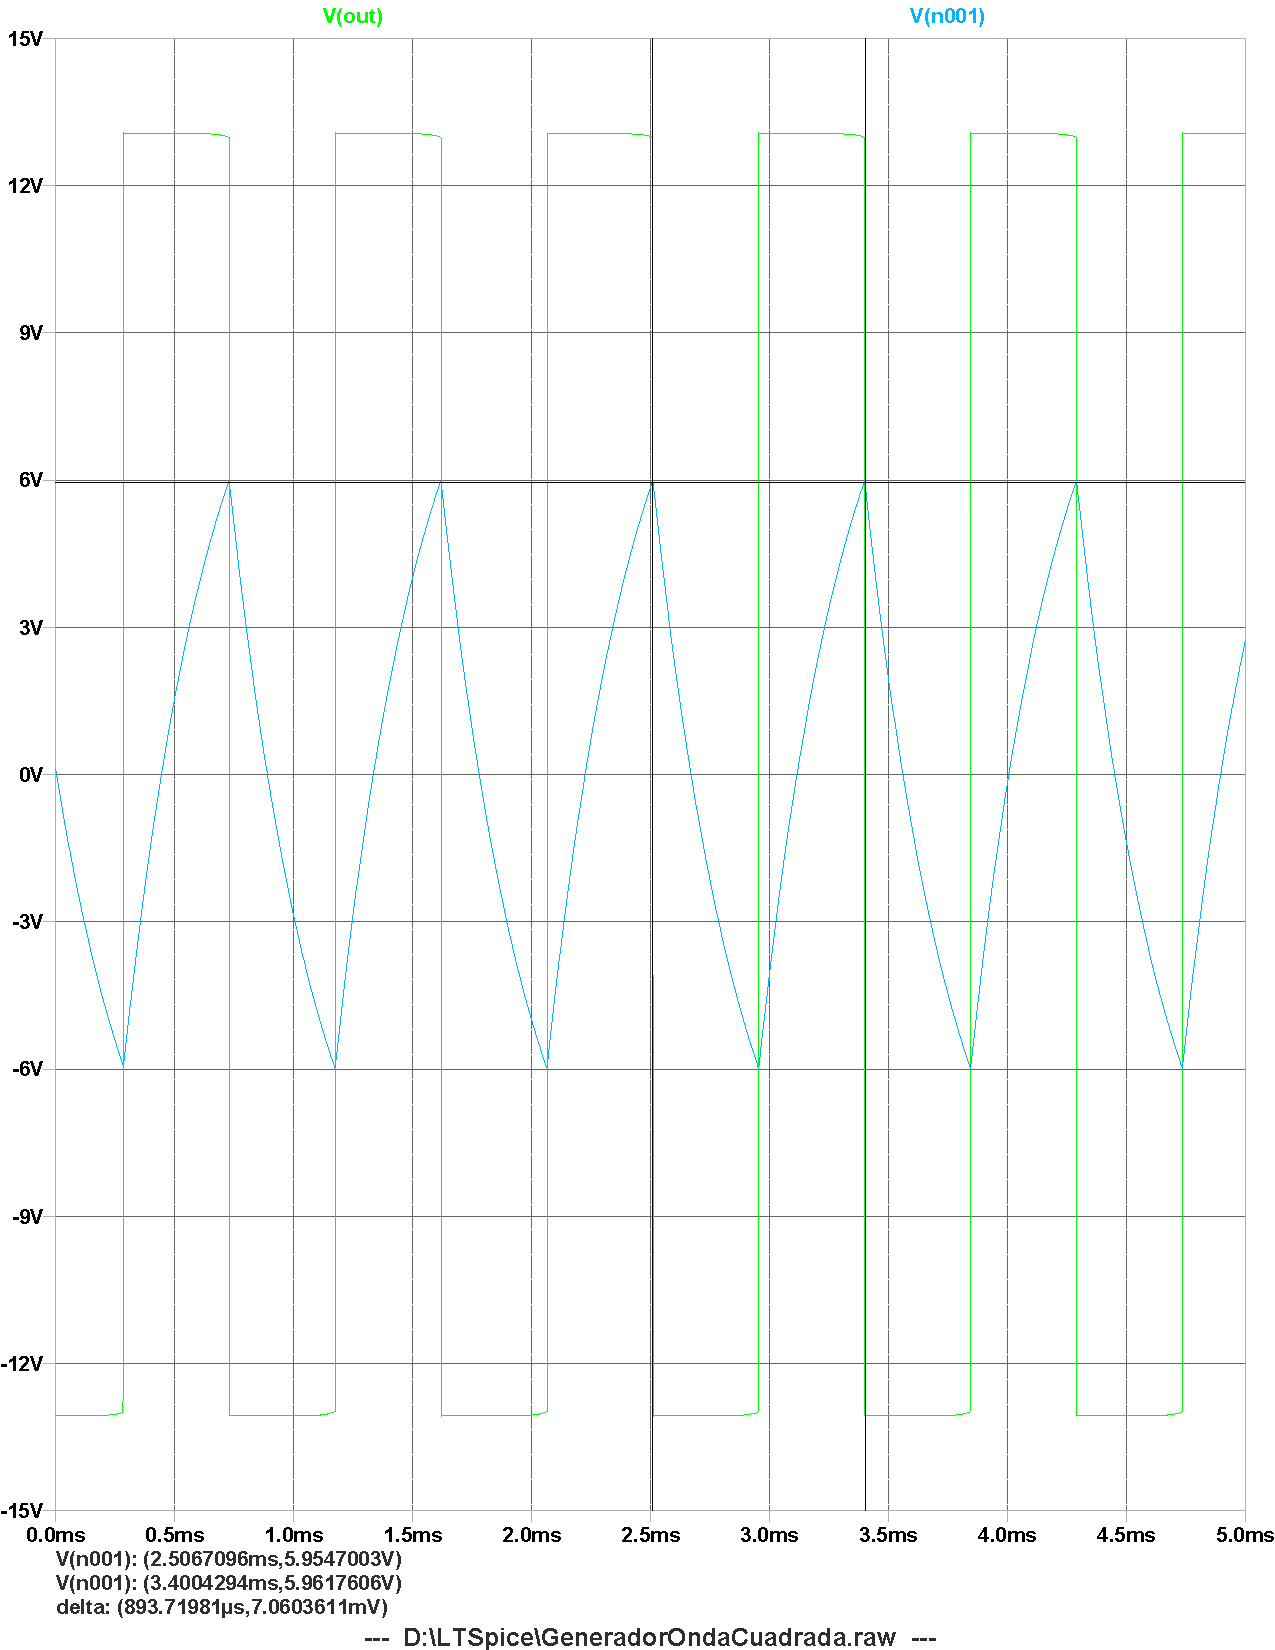
\includepdf[]{GeneradorOndacuadradaPlot}

\noindent A continuación se muestra los resultados obtenidos con el osciloscopio
\begin{figure}[H]
	\centering
	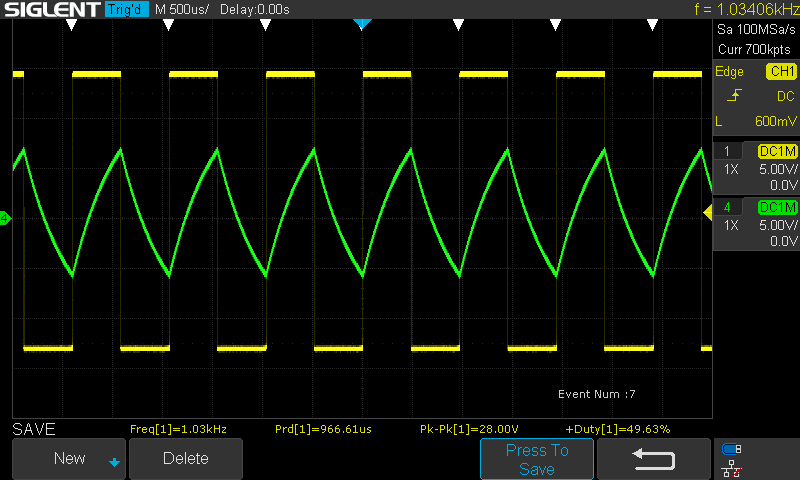
\includegraphics[width=\textwidth]{SDS00006}
	\caption{}	
	\label{fig:figura3}
\end{figure}

\begin{figure}[H]
	\centering
	
\includegraphics[height=15cm, angle=90]{circuito}
	\caption{}	
	\label{fig:figura4}
\end{figure}

\end{document}